%%%%%%%%%%%%%%%%%%%%%%%%%%%%%%%%%
%
%       EXERCÍCIO
%
%%%%%%%%%%%%%%%%%%%%%%%%%%%%%%%%%

\ifdefstring{\atividade}{prova}{%
    \renewcommand{\valorquestao}{\ValorQ\ pontos}
}%

\begin{exercicioBanco}[\valorquestao]
O gráfico apresenta a taxa de desemprego (em \%) para o período de março de 2008 a abril de 2009, com base nos dados observados nas regiões metropolitanas de Recife, Salvador, Belo Horizonte, Rio de Janeiro, São Paulo e Porto Alegre.

\begin{center}
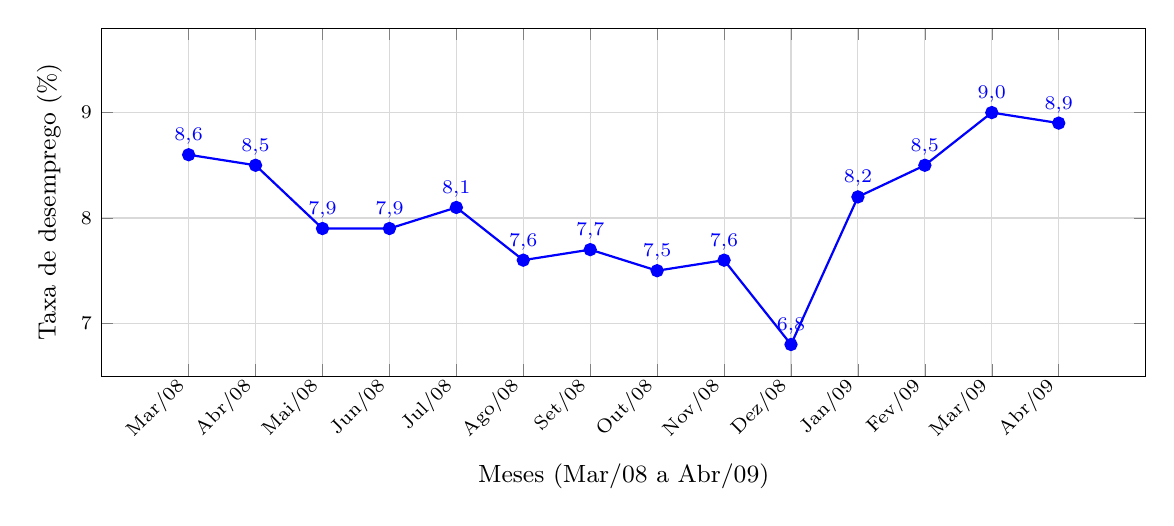
\begin{tikzpicture}
\begin{axis}[
    x=0.85cm, % Estica a distância entre cada ponto no eixo X (ajuste esse valor se quiser mais/menos esticado)
    height=6cm, % Define a altura do eixo Y
    xlabel={Meses (Mar/08 a Abr/09)},
    ylabel={Taxa de desemprego (\%)},
    ymin=6.5, ymax=9.8,
    xtick={1,...,14},
    xticklabels={
        Mar/08,Abr/08,Mai/08,Jun/08,Jul/08,Ago/08,Set/08,Out/08,
        Nov/08,Dez/08,Jan/09,Fev/09,Mar/09,Abr/09},
    x tick label style={rotate=45, anchor=east, font=\scriptsize},
    y tick label style={font=\scriptsize},
    label style={font=\small},
    grid=both,
    major grid style={gray!30},
    minor grid style={gray!15}
]
\addplot[
    color=blue,
    mark=*,
    thick,
    nodes near coords,
    point meta=explicit symbolic,
    every node near coord/.append style={font=\scriptsize, anchor=south}
] coordinates {
    (1,8.6) [8,6]
    (2,8.5) [8,5]
    (3,7.9) [7,9]
    (4,7.9) [7,9]
    (5,8.1) [8,1]
    (6,7.6) [7,6]
    (7,7.7) [7,7]
    (8,7.5) [7,5]
    (9,7.6) [7,6]
    (10,6.8) [6,8]
    (11,8.2) [8,2]
    (12,8.5) [8,5]
    (13,9.0) [9,0]
    (14,8.9) [8,9]
};
\end{axis}
\end{tikzpicture}
\end{center}

A mediana dessa taxa de desemprego, no período de março de 2008 a abril de 2009, foi de quanto?

\end{exercicioBanco}

